\documentclass[a4paper,14pt]{extarticle}
\usepackage[T2A]{fontenc}
\usepackage[utf8]{inputenc}
\usepackage[english,russian]{babel}
\usepackage{amsmath,amsfonts,amsthm, mathtools}
\usepackage{amssymb}
\usepackage{icomma}
\usepackage{graphicx}
\usepackage{wrapfig}
\RequirePackage{longtable}
\newcommand*{\hm}[1]{#1\nobreak\discretionary{}
	{\hbox{$\mathsurround=0pt #1$}}{}}

\usepackage{soulutf8} 
\usepackage{geometry}
\geometry{top=20mm}
\geometry{bottom=20mm}
\geometry{left=20mm}
\geometry{right=20mm}


\begin{document}
\begin{center}
	\textit{Федеральное государственное автономное образовательное\\ учреждение высшего образования }
	
	\vspace{0.5ex}
	
	\textbf{«Московский физико-технический институт\\ (национальный исследовательский университет)»}
\end{center}

\vspace{10ex}


\begin{center}
	\vspace{13ex}
	
	\textbf{Лабораторная работа №1.1.4}
	
	\vspace{1ex}
	
	по курсу общей физики
	
	на тему:
	
	\textbf{\textit{<<Измерение интенсивности радиационного фона>>}}
	
	\vspace{30ex}
	
	\begin{flushright}
		\noindent
		\textit{Работу выполнил:}\\  
		\textit{Никифоров Дмитрий \\(группа Б02-205)}
	\end{flushright}
	\vfill
	Долгопрудный \\ \today
	
	%\setcounter{page}{1}
\end{center}

	
	
		• Цель работы: применение методов обработки экспериментальных данных для изучения статистических закономерностей при измерении интесивности радиационного фона
	
	
	В работе исппользуется: счетчик  Гейгера-Мюллера(СТС-6), блок питания, компьютер с интерфейсом связи со счетчиком.
	\newline
	
	• Теоретические сведения:
	\newline
	
	Значительную часть радиационного фона составляет поток космических частиц, изменяющийся со временем случайным образом.
	Космические лучи разделяют на первичные - поток стабилных частиц, имеющих большую кинетическую энергию ($10^{9} - 10^{21}$ эВ) и вторичные, которые возникают при взаимодействии первичных с атмосферой Земли и составляют основную часть космичексих лучей, доходящих до поверхности Земли.
	Установлено, что в космическом пространстве поток частиц изотропен.
	\newline
	
	
	• Устройство счетчика Гейгера-Мюллера.
	\newline
	
	Счетчик, используемый в данной работе (СТС-6), представляет собой  наполненный газом сосуд с двумя электродами:
	катодом(тонкостенным металлическим цилиндром) и анодом(тонкой нитью, натянутой вдоль оси циллиндра).
	На электроды подается напряжение 400 В.
	Частицы космических лучей ионизируют газ, находящийся в счетчике, а также выбивают электроны из его стенок; таким образом появляются свободные электроны. Под действием электрического поля между электродами электрон разгоняется и врезается в другие атомы, вибивая из них новые электроны.Развиваясь лавинообразно, этот процесс завершается образованием в межэлектродном пространстве электронно-ионного облака, резко увеличивающего его проводимость. По
	существу, при попадании в счетчик Гейгера частицы в нём вспыхивает (зажигается) самостоятельный
	газовый разряд, видимый (если баллон прозрачный) даже простым глазом.
	\newline
	
	
	
	
	• Основные расчётные формулы:
	\newline
	
	Ошибка единичного измерения $\sigma = \sqrt{n}$. (В данном эксперименте n - это число импульсов)
	
	В полосе $n\pm\sqrt{n}$ лежит 68\% точек.
	
	Ошибка среднего $\overline{\sigma} = \sqrt{\overline{n}}$.
	
	Стандартное отклонение $\sigma = \dfrac{\overline{\sigma}}{\sqrt{N}}$, где N - это количество измерений.
	\newline
	
	
	\newpage
	
	
	• Графики:
	\newline
	
	\begin{wrapfigure}[10]{1}{0.6\linewidth}
		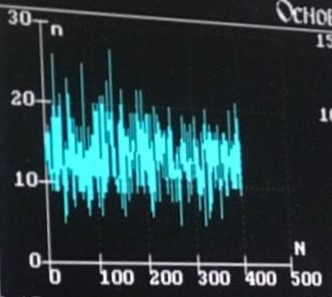
\includegraphics[width= 10cm, height= 8cm]{1.jpg}
		\caption{Основной эксперимент}
	\end{wrapfigure}

	
	По этому графику через равные промежутки времени измеряем полосу, в которую попадают все точки, и  укорачиваем ее в $\frac{2}{3}$ раза, а потом делим пополам. Это и будет наша ошибка. Также по графику можем оценить среднее значение и сравнить его с реальным с помощью графика ниже.
	\newline
	\bigskip
	\\
	\\
	\\
	\\
	\\
	
	
	
	
	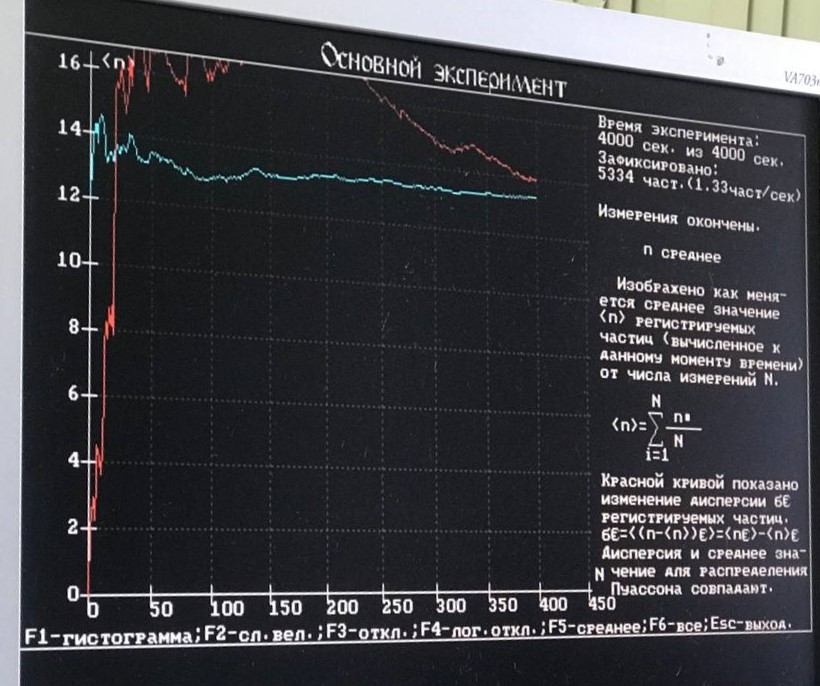
\includegraphics[width= 10cm, height=8cm]{2.jpg}
	
	
	
	\newpage
	\begin{wrapfigure}[19]{1}{0.6\linewidth}
		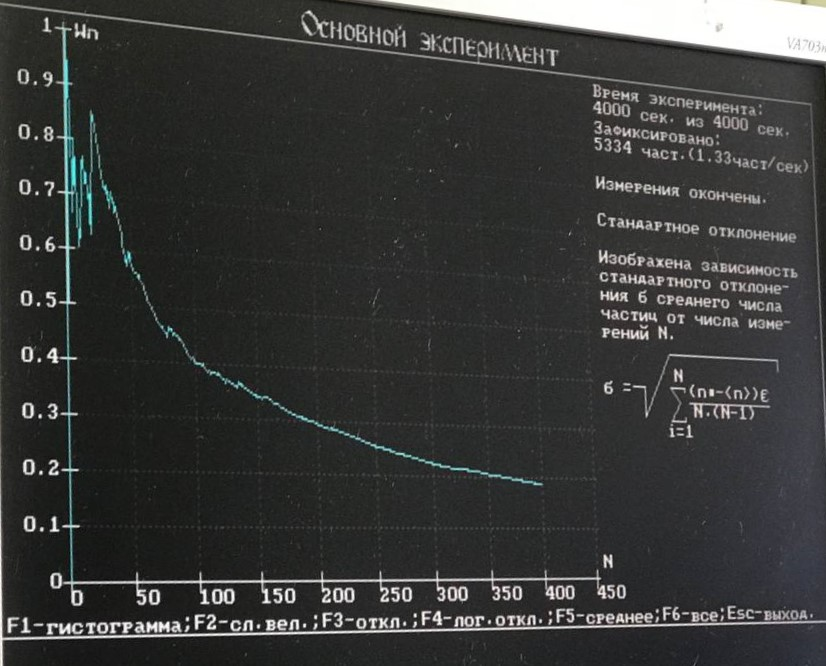
\includegraphics[width= 10cm, height= 8cm]{3.jpg}
		\caption{Стандартное отклонение}
		
		
		
		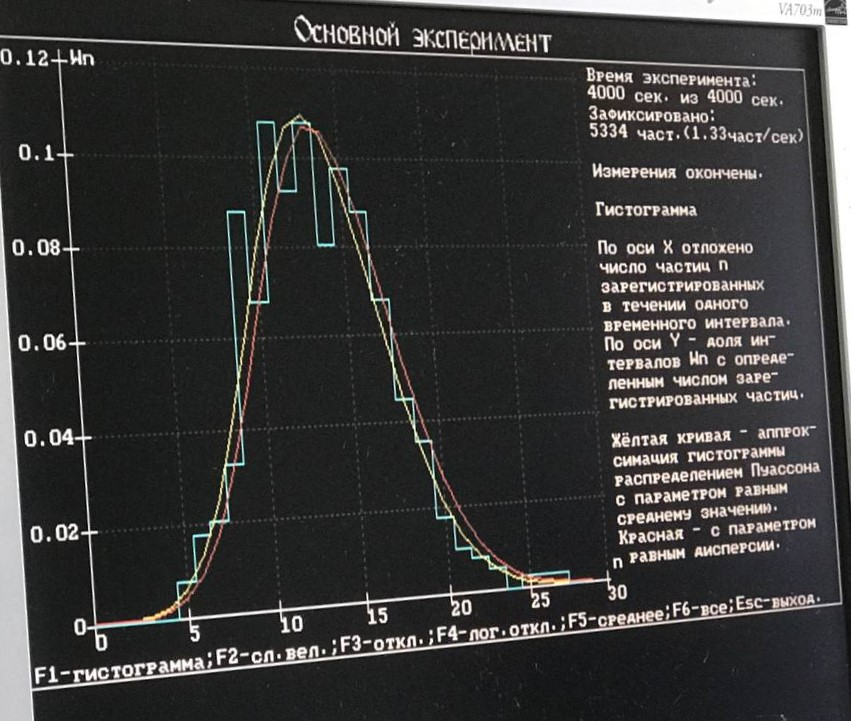
\includegraphics[width= 10cm, height= 8cm]{4.jpg}
		\caption{Гистограмма}
	\end{wrapfigure}
	

	Опираясь на предыдущие данные, которые мы уже получили(ошибку среднего), вычисляем стандартное отклонение по формуле $\sigma = \dfrac{\overline{\sigma}}{\sqrt{N}}$ и сравниваем с реальным по графику.
	\newline
	\bigskip
	\\
	\\
	\\
	\\
	\\
	По гистограмме видим на какое число импульсов приходится максимум и убеждаемся в нормальности распределения нашей случайной величины, так как кривая красиво ложится на гауссиану.
	\newline
	\bigskip
	\\
	\\
	\\
	\\
	\\
	\\
	\\
	\newpage
	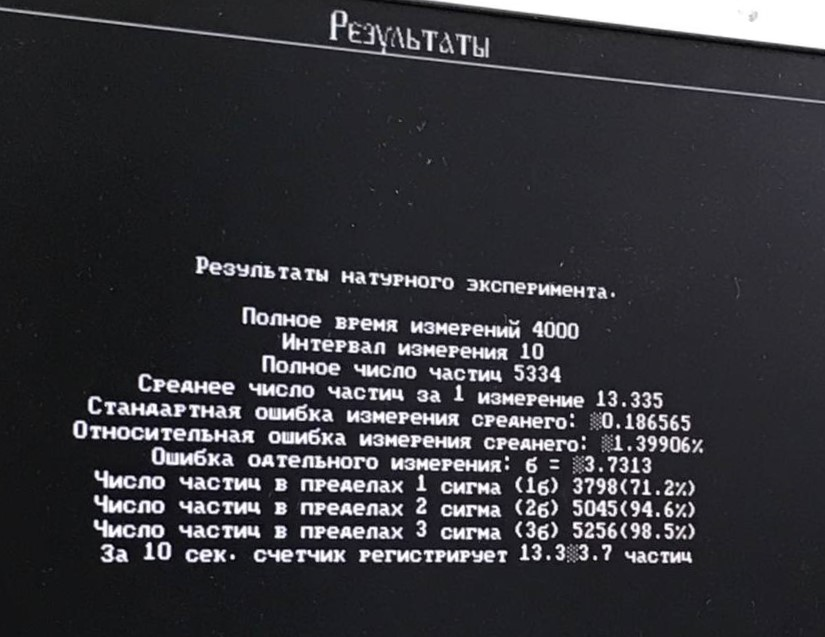
\includegraphics[width= 7cm, height= 5cm]{5.jpg}
	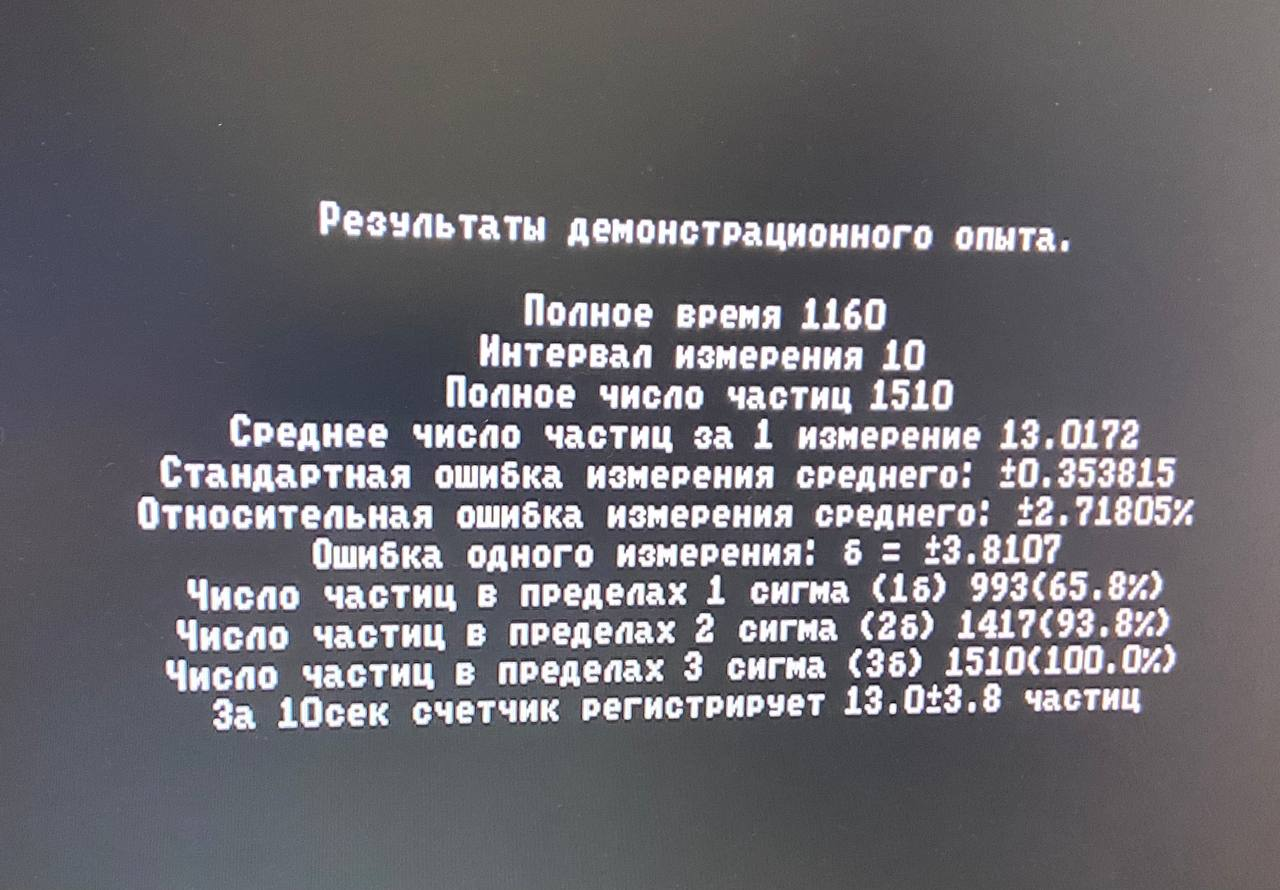
\includegraphics[width= 7cm, height= 5cm]{7.jpg}
	
	
	Сравнив результаты основного и демонстрационного опыта, можно заметить, что данные получились довольно похожими, даже несмотря на меньшее количество измерений во втором опыте. Из этого можно сделать вывод, что распределение нормальное, а ошибка случайная.
	


	• Результаты измерений и обработка данных:
	
	
	\begin{center}
		
		\begin{tabular}{|c|c|c|c|c|c|}
			\hline
			Количество измерений & 80 & 160 & 240 & 320 & 400  \\ \hline
			Оценка ошибки по полосе & 2.5 & 2.5 & 2.0 & 3.0 & 3.2   \\ \hline
			Оценка среднего & 13 & 13 & 13 & 13 & 13   \\ \hline
			Реальное среднее & 13.1 & 13.4 & 13.6 & 13.5 & 13.5   \\  \hline
			Оценка ошибки среднего & 3.5 & 3.5 & 3.5 & 3.5 & 3.5  \\ \hline
			Оценка стандартного отклонения & 0.28 & 0.2 & 0.13 & 0.17 & 0.16  \\  \hline
			Реальное стандартное отклонение & 0.45 & 0.32 & 0.28 & 0.22 & 0.19   \\ \hline
			
		\end{tabular}
	\end{center}
	%\caption{Заголовок мог быть и здесь}
	
	
	
	
	• Заключение:
	\newline
	
	Нам удалось измерить интенсивность радиационного фона. Мы применили статистические методы для анализа данных и пришли к выводу, что радиационный фон стабилен. Также нам удалось довольно хорошо оценить погрешности, среднее значение и стандартное отклонение.
\end{document}